\chapter{Calibration}

Alterations of the laboratory environment combined with the exchange of
components from the original setup made it necessary to recalibrate the setup.
In this chapter we want to document the calibration steps required to
reproduce the claimed results.

\section{Fiber Coupling}

The visually shielded section of the setup, used to reduce the output power
of the laser source, is optically paired with the open section for beam
deflection via a \gls{smf} that only permits two orthogonal polarization and
a single gaussian mode. By tuning the polarisator inside the power
reduction section we can try to match one of the orthogonal polarization
modes supported by the \gls{smf}. Polarization discrepancies cause the
polarization inside the \gls{smf} to oscillate with vibrations or changes in
temperature, henceforth it is key to couple polarization modes in order to
ensure a stable operation.

\begin{figure}[h]
  \centering
  \includegraphics[height=6cm]{example-image-a}
  \caption{Intensity oscillations observed through the oscilloscope when
  heating the \gls{smf}.}
  \label{fig:fibercoup}
\end{figure}

A strategy proven to find an approximate polarization match between the
laser beam and the \gls{smf} is presented. In addition to the setup described
in \cref{sec:powerbox} and \cref{sec:deflection} an oscilloscope and a hot
air gun were used.

\begin{enumerate}
  \item Connect the photodiode to the oscilloscope and use a coarse time
    scale (i.e. \SI{2}{\second}).
  \item Apply appropriate laser safety glasses and inform present personal
    of the imminent danger.
  \item Open the cover of the power reduction setup.
  \item Apply heat to the \gls{smf} through the hot air gun, alternatively
    you can try to move the fiber.
  \item The photodiode signal should start to oscillate. Tune the polarizor
    inside the power reduction subject to minimizing the oscillation.
\end{enumerate}

The oscillations occur as the polarization circulates inside the fiber and
will stop at some point when a new equilbrium has been established. In this
case remove the heat or mechanical stress on the fiber and wait before you
reapplying new impetus.

\section{Beam Alignment}

Beams that pass off-centered through spherical lenses experience optical
aberrations, additionally uncentered beams may cause further optical defects
from reflections or clipping at boundaries. Since most changes to the optical
setup outdate the previous beam alignment, hence making the realignment
a rather frequent procedure, we want to showcase what worked well for us.

As auxilliaries we used a pair of iris diaphragms that can be placed in front
of the lens mounts as a screen (i.e. a white sheet of hard paper). By placing
both iris diaphragms towards the incident beam on two successive lenses we
we can visually find a center reference point by inspecting the symmetry of
the iris illumination at different pinhole diameters.

\begin{figure}[h]
  \centering
  \minipage{0.45\textwidth}
    \includegraphics[width=\linewidth]{example-image-a}
    \caption{Typical beam alignment situation involving the mirrors M1, M2 and
    lenses L1, L2.}
    \label{fig:beamalign:setup}
  \endminipage
  \hfill
  \minipage{0.45\textwidth}
    \includegraphics[width=\linewidth]{example-image-a}
    \caption{Unaligned beam missing the iris pinhole and suggested mirror
    adjustments.}
    \label{fig:beamalign:iris}
  \endminipage
  \hfill
\end{figure}

\Cref{fig:beamalign:iris} shows a misaligned beam hits the iris diaphragms
and how to adjust the mirror angles. It should be noted that this is an
iterative process.

\section{Camera Focus}

Finally we had to reposition the camera to focus the incoming beam on the
\gls{ccd} sensor of the camera. Finding the precise focus position is not an
easy undertaking. There is no sharp focal spot but rather a focal area,
however outside the focal area no image can be seen.

We followed the procedure described in \cite{Hertlein2017} that consists of
extracting the camera rail with its lens and focusing it on a far distant
object.

\begin{figure}[ht]
  \centering
  \minipage{0.5\textwidth}
  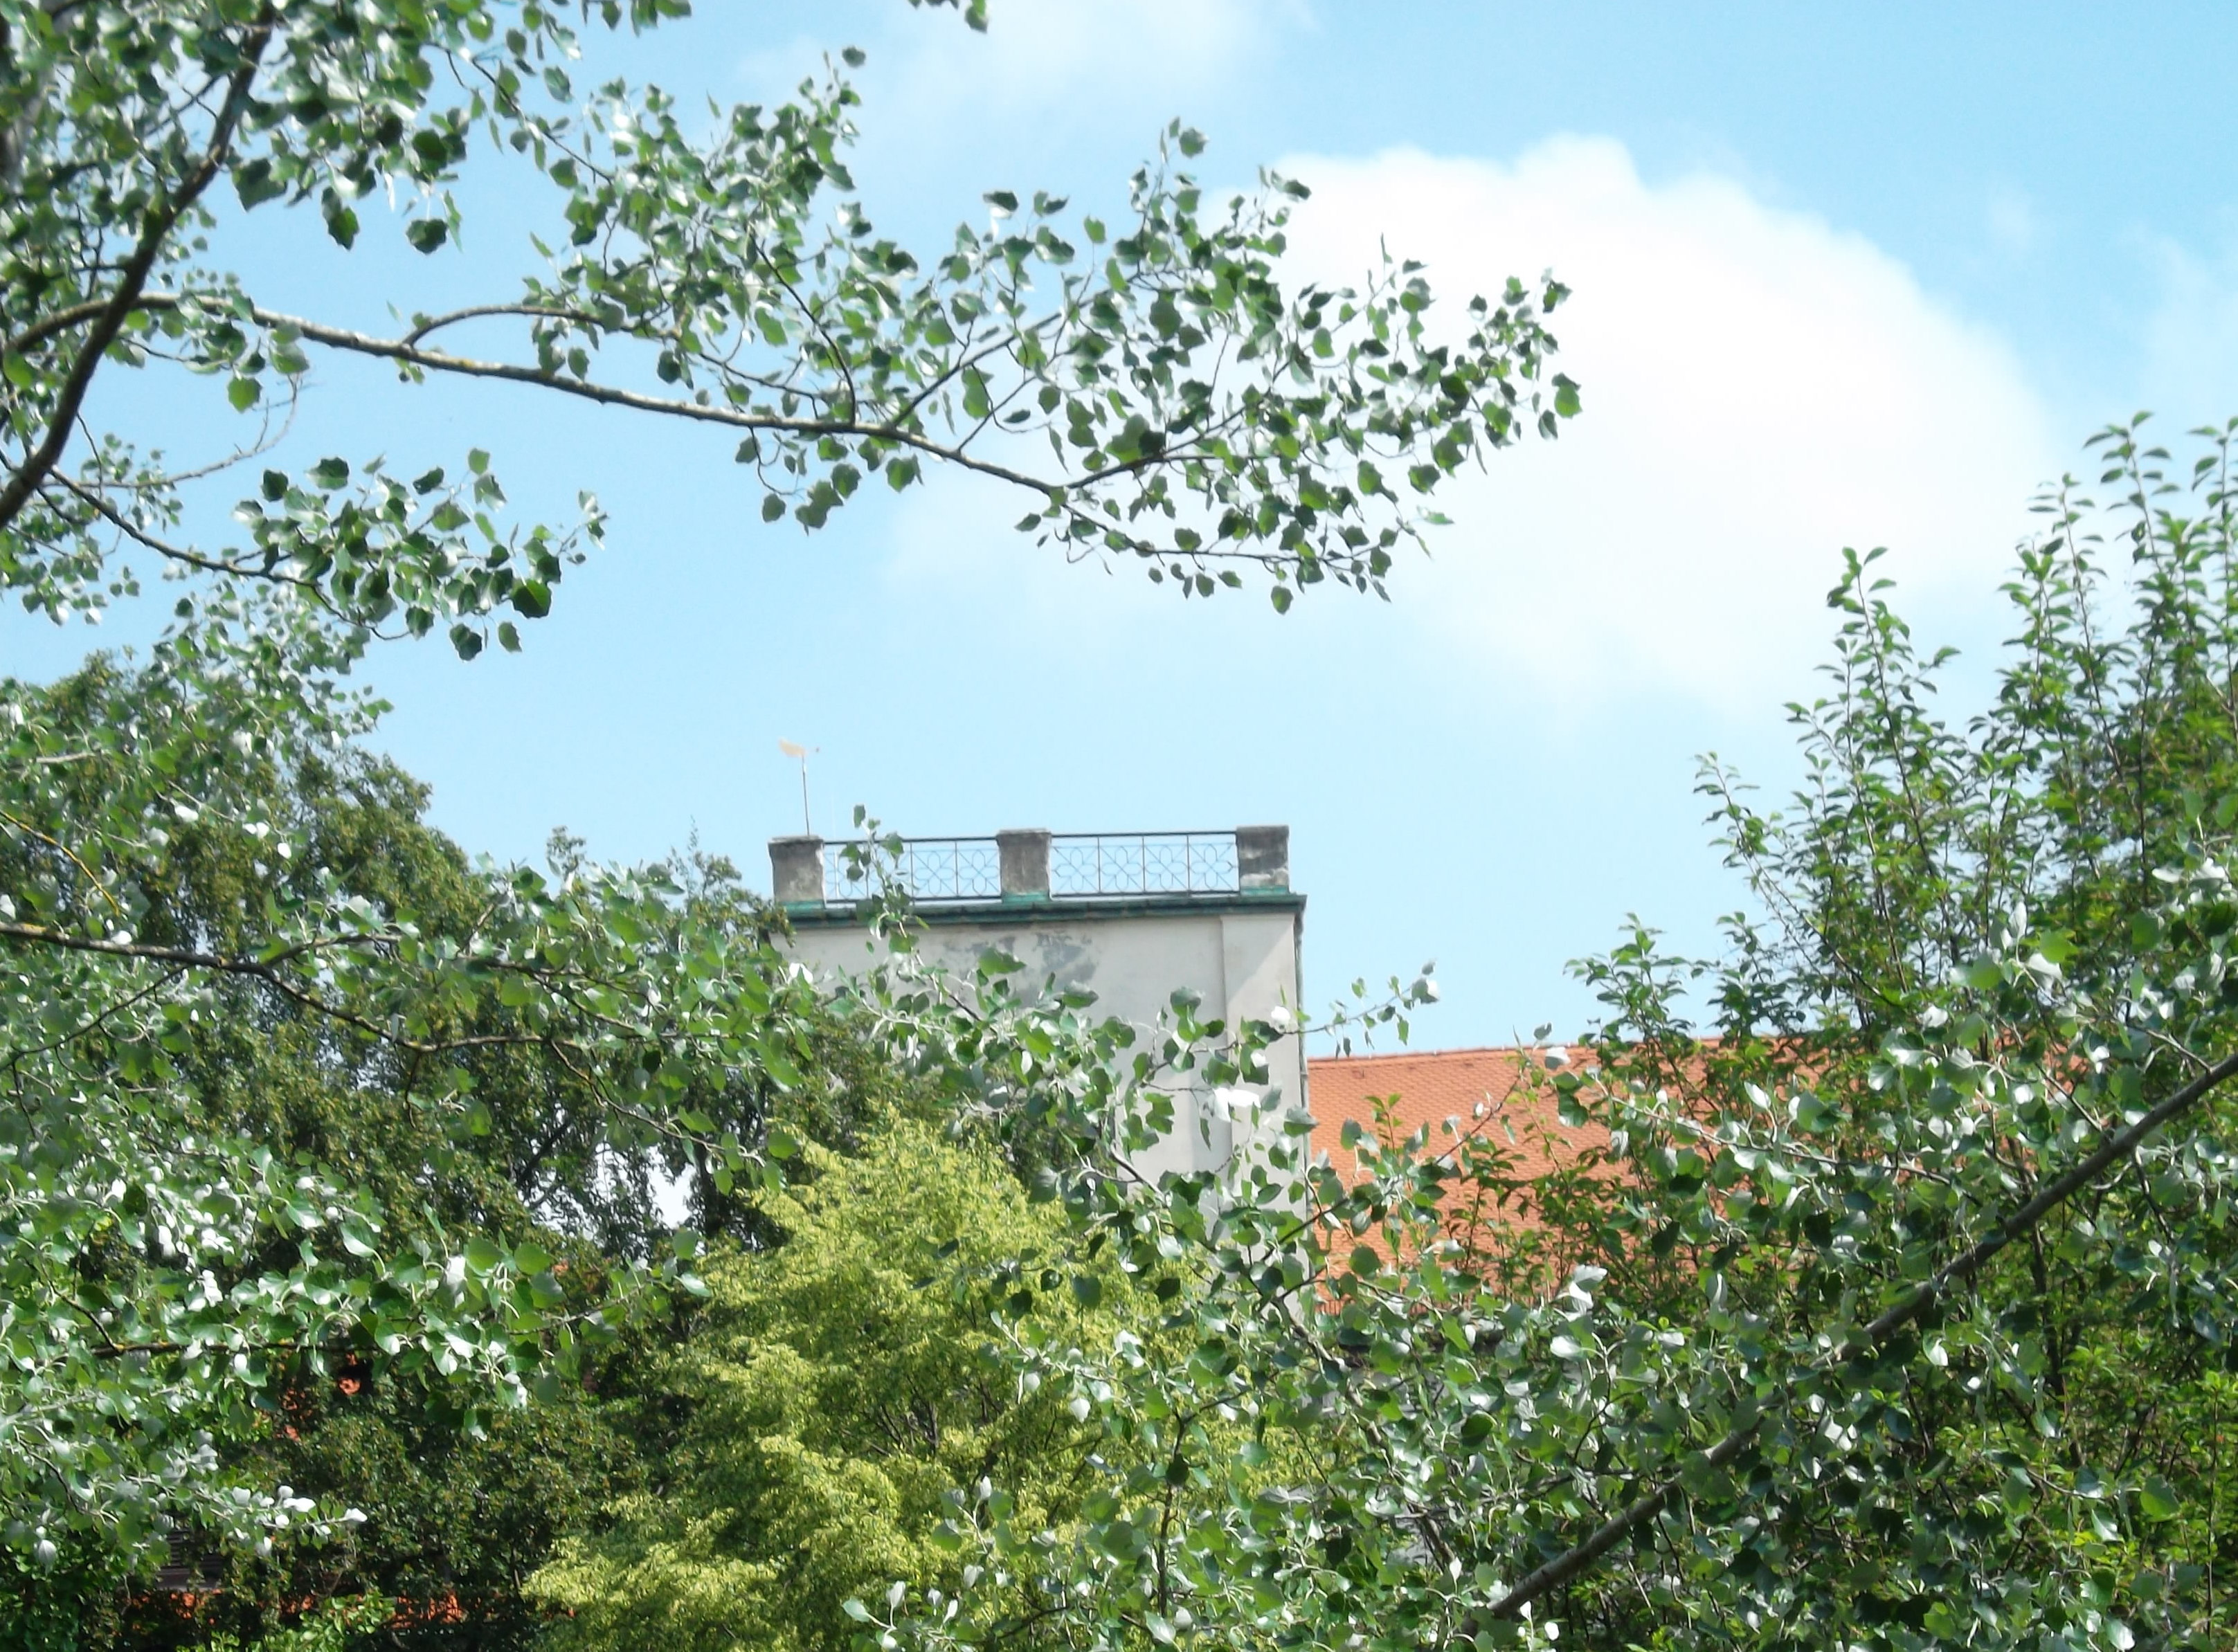
\includegraphics[width=\linewidth]{images/focus/view3.jpg}
    \caption{The view as seen from the window towards the university tower
      captured with a normal digital camera.}
    \label{fig:camerafocus:view}
  \endminipage
  \hfill
  \minipage{0.45\textwidth}
    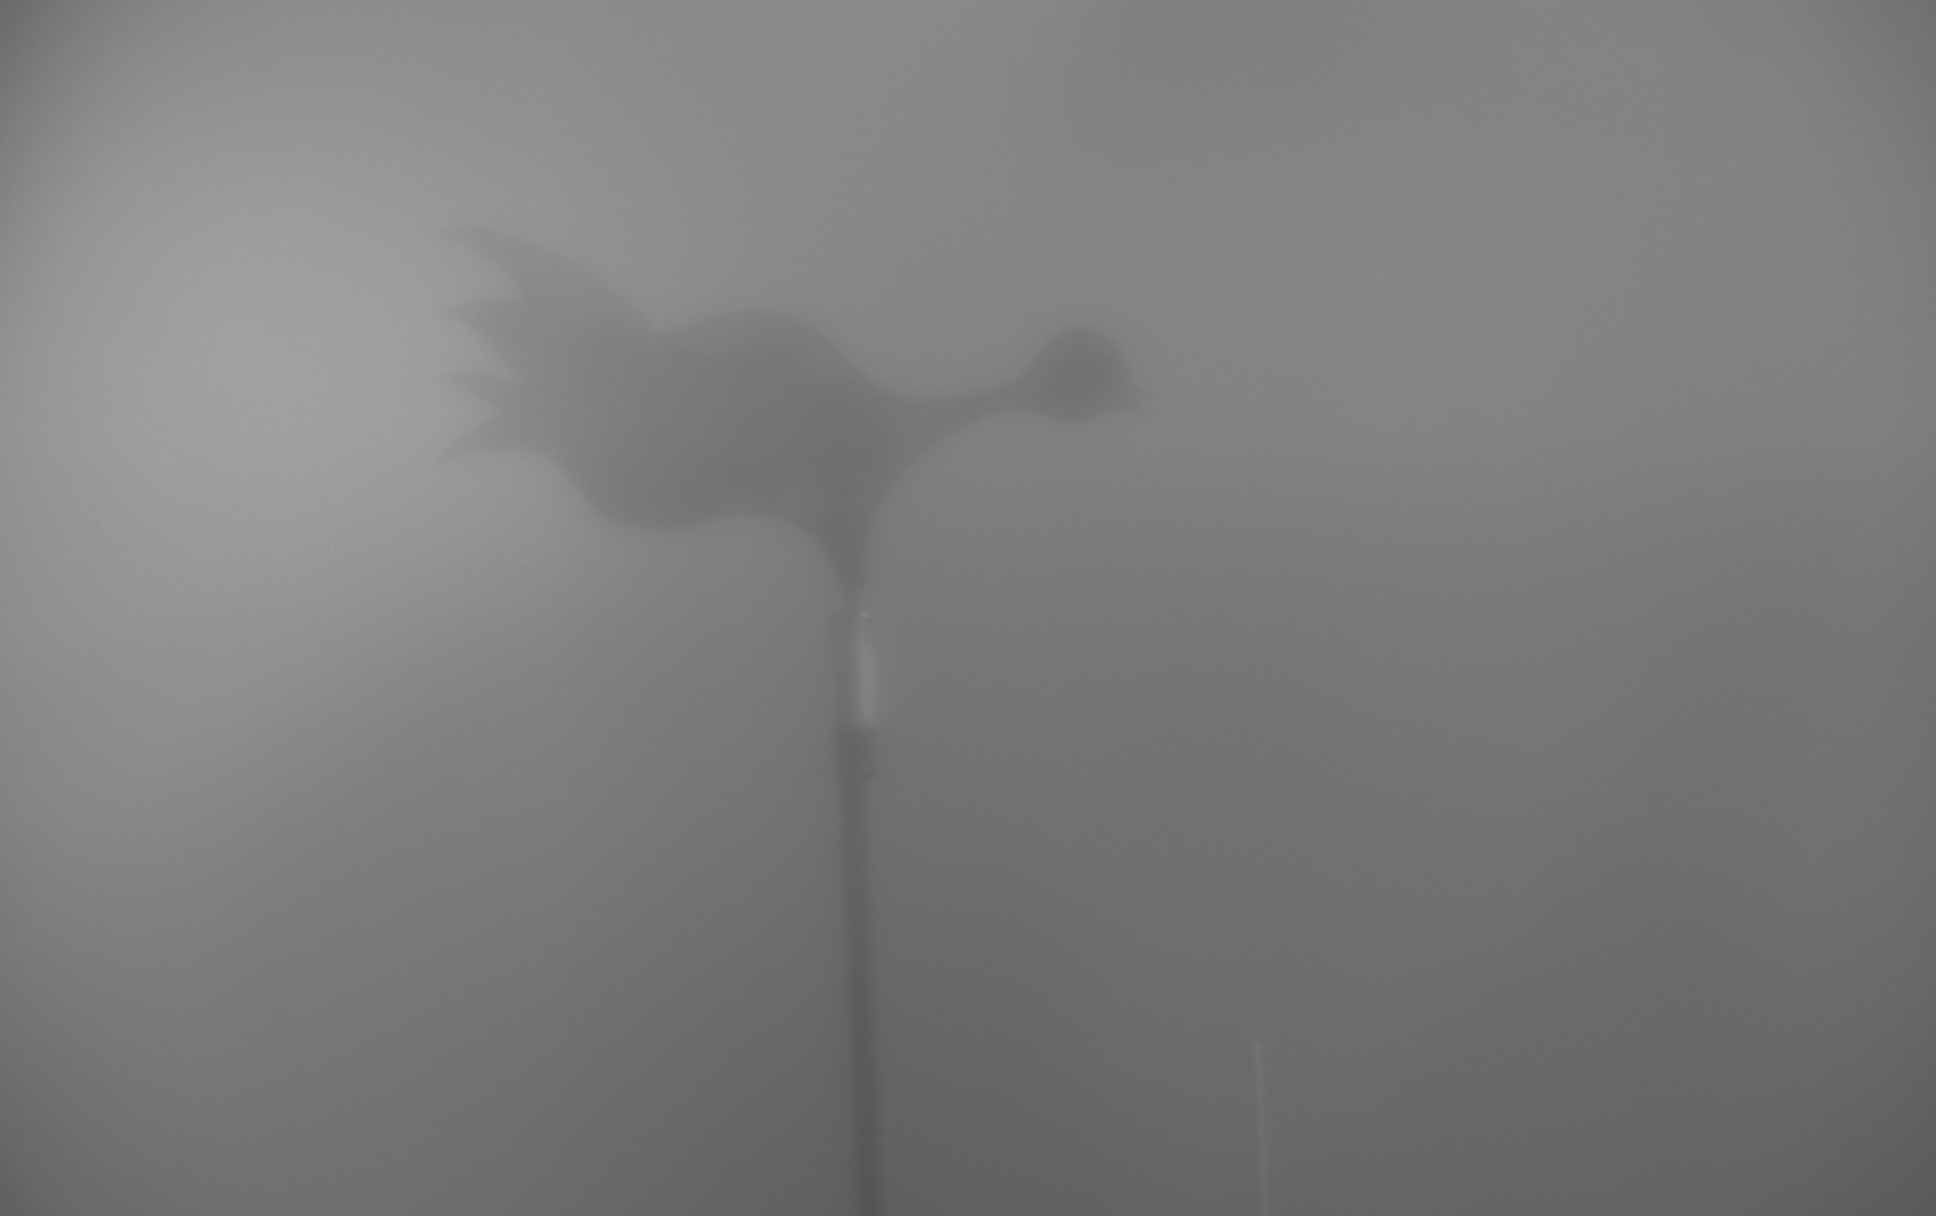
\includegraphics[width=\linewidth]{images/focus/focus3.jpg}
    \caption{Focused camera with view on the weather cock on the top of the
    university tower.}
    \label{fig:camerafocus:cock}
  \endminipage
  \hfill
\end{figure}

\section{Assessment}

With the previously described calibration steps in place we can assess the
final quality of the beam with an image capture of the \gls{ccd} camera in the
aligned setup \cref{sec:deflection}.

\begin{figure}[h]
  \centering
  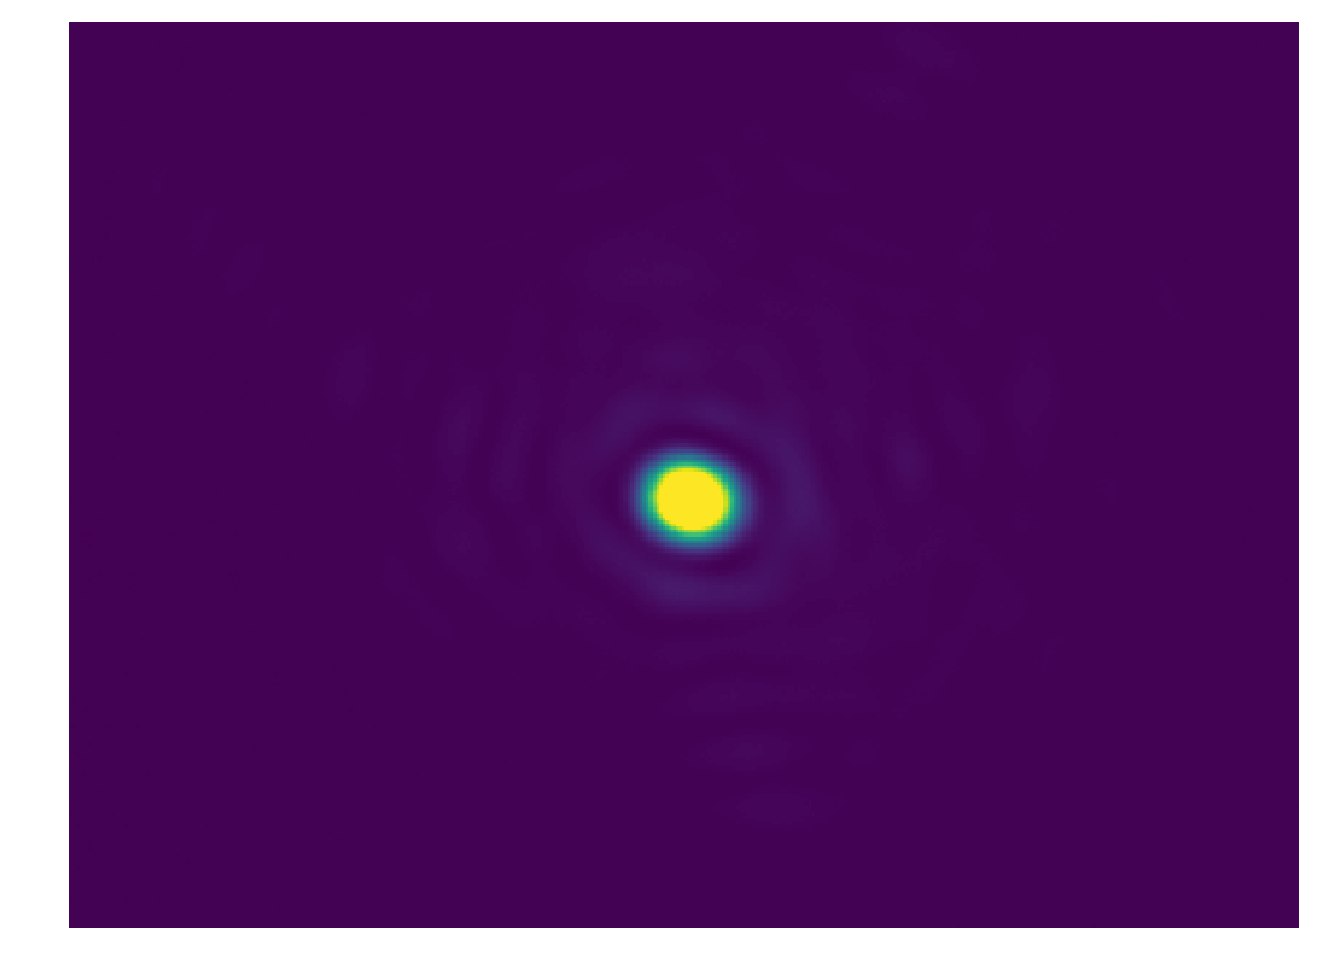
\includegraphics[width=.5\textwidth]{images/camera/profile2d.pdf}
  \caption{Image detail from the captured beam with the \gls{ccd} camera.}
  \label{fig:beamprofile:2d}
\end{figure}

The two dimensional beam profile shows the characteristical two dimensional
gaussian distribution with diffraction rings caused by beam clipping at
finite apertures as described in \cite{Hertlein2017}.

\begin{figure}[h]
  \centering
  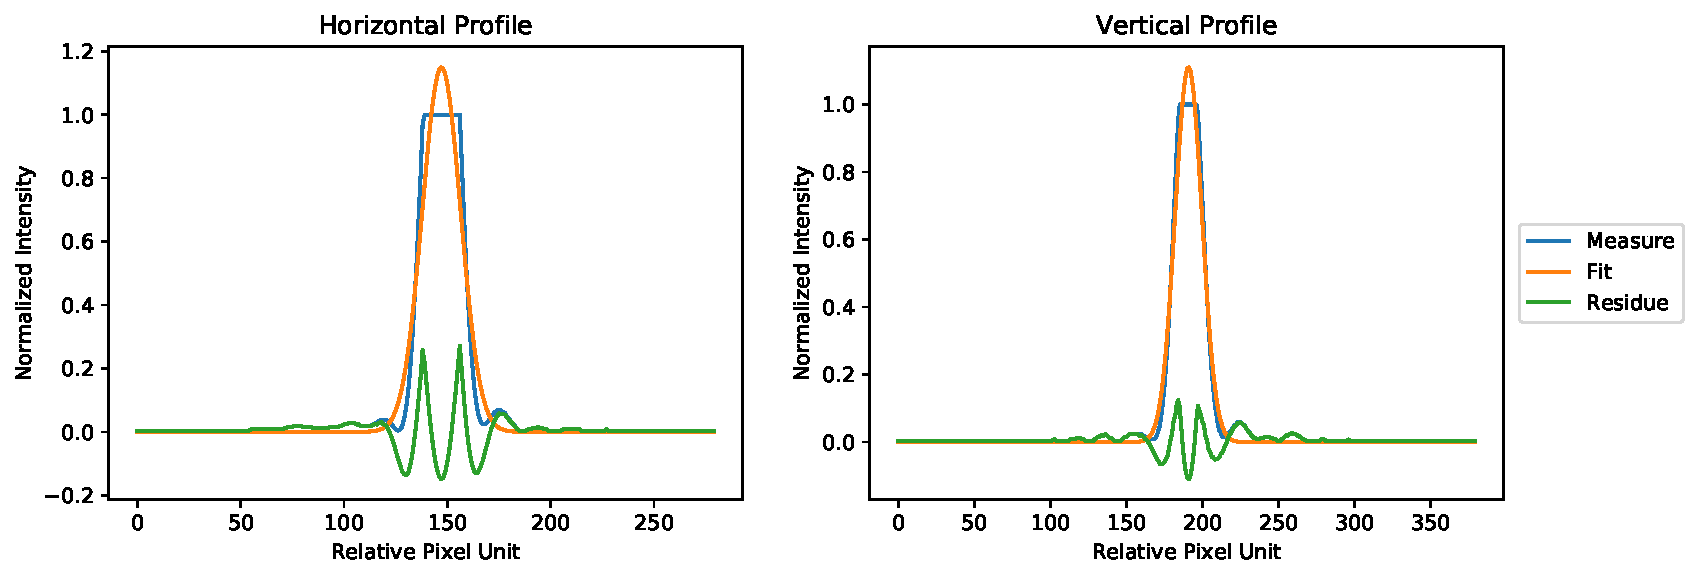
\includegraphics[width=\textwidth]{images/camera/profile1d.pdf}
  \caption{1D horizontal and vertical profile extracted from the center of
    the image detail in \cref{fig:beamprofile:2d} with fitted gaussian curve
  and residue.}
  \label{fig:beamprofile:1d}
\end{figure}

By inspecting the one dimensional profiles with fitted gaussian and residue
we again confirm conclusions drawn in \cite{Hertlein2017}. The clipped top
of the measured intensity originates from the saturated pixels of the
\gls{ccd} camera and can be ignored. We further observe a slight assymmetry
at the diffraction rings. Overall the shown profiles can be considered to
confirm a good alignment.
